

\documentclass{article}
\usepackage[utf8]{inputenc}
\usepackage{authblk}
\usepackage{setspace}
\usepackage[margin=1.25in]{geometry}
\usepackage{graphicx}
\graphicspath{ {./figures/} }
\usepackage{subcaption}
\usepackage{amsmath}
\usepackage{lineno}
\usepackage{booktabs}% pour les table depuis R
\usepackage{makecell}
\linenumbers

%%%%%% Bibliography %%%%%%

\usepackage[
    style=nejm, 
    citestyle=numeric-comp,
    sorting=none, 
    backend=biber]{biblatex}

\addbibresource{treeModel.bib}

%%%%%% Title %%%%%%
% Full titles can be a maximum of 100 characters, including spaces. 
% Title Format: Use title case, capitalizing the first letter of each word, except for certain small words, such as articles and short prepositions
\title{From Local Actors to Leaf Protectors: A Collaborative Modeling Approach for Rethinking Tree Management and Protection Measures in Senegal's Groundnut Basin}

%%%%%% Authors %%%%%%
% Authors should be listed in order of contribution to the paper, by first name, then middle initial (if any), followed by last name.
% Authors should be listed in the order in which they will appear in the published version if the manuscript is accepted. 
% Use an asterisk (*) to identify the corresponding author, and be sure to include that person’s e-mail address. Use symbols (in this order: †, ‡, §, ||, ¶, #, ††, ‡‡, etc.) for author notes, such as present addresses, “These authors contributed equally to this work” notations, and similar information.
% You can include group authors, but please include a list of the actual authors (the group members) in the Supplementary Materials.
\author[1,2,6*$\dag$]{E. Delay}
\author[1,2,4$\dag$]{L. Broutin}
\author[1,2]{A. Fallot}
\author[3]{A. Perrotton}
\author[4]{A. Gonin}
\author[5]{D. Masse}


%%%%%% Affiliations %%%%%%
\affil[1]{CIRAD, UMR SENS, F-34398 Montpellier, France.}
\affil[2]{SENS, CIRAD, IRD, Université de Paul Valéry Montpellier 3, Montpellier, France.}
\affil[3]{Forêts et Sociétés, Univ Montpellier, CIRAD, Montpellier, France.}
\affil[4]{Université Paris Nanterre, Laboratoire LAVUE, FR.}
\affil[5]{IRD, Eco\&Sols, Abidjan, Côte d’Ivoire.}
\affil[6]{UMI UMMSCO,  Université Cheick Anta Diop, Dakar, Sénégal.}
\affil[*]{Address correspondence to: etienne.delay@cirad.fr}
\affil[$\dag$]{These authors contributed equally to this work.}

%%%%%% Date %%%%%%
% Date is optional
\date{}

%%%%%% Spacing %%%%%%
% Use paragraph spacing of 1.5 or 2 (for double spacing, use command \doublespacing)
\onehalfspacing

\begin{document}

\maketitle

%%%%%% Abstract %%%%%%
\begin{abstract}

    How can a participatory simulation model contribute to understanding the socio-ecological dynamics and fostering innovative strategies for sustainable management of trees, crops, and pastoralism in the peanut basin?

    In the agro-pastoral zones, the Sahelian ecosystems have undergone significant degradation, characterized by a reduction in tree cover, as a consequence of the droughts in the 1960s and 1990s. The peanut basin stands out for its positive interrelationships between trees, crops, and pastoralism. However, the regeneration of the Faidherbia park has declined since the major droughts. Through collaborative efforts with agro-pastoral farmers, we have developed a simulation model -- The SAFIRe model : Simulation of Agents for Fertility, Integrated Energy, Food security, and Reforestation-- that aims to unravel the complex social and ecological dynamics at play and explore potential strategies in partnership with local communities.

    By exploring the results of the model co-designed with local stakeholders, we have identified more effective management strategies, as per the request of the local actors. However, more importantly, we have collectively questioned the conditions for improving tree cover and the viability of the socio-ecosystem, particularly in relation to the demand for firewood and local cereal for sustenance. This has prompted the stakeholders to engage in community-wide discussions and transform agro-pastoralists into leaf protectors.

\end{abstract}

%%%%%% Main Text %%%%%%

\section{Introduction}
Your manuscript should contain all of the numbered sections specified in this template: Introduction, Results, Discussion, Materials and Methods.

The manuscript should start with a brief introduction that lays out the problem addressed by the research and describes the paper’s importance. The scientific question being investigated should be described in detail. The introduction should provide sufficient background information to make the article understandable to readers in other disciplines and provide enough context to ensure that the implications of the experimental findings are clear. 

% %%%%% Citations in the text %%%%%%
% \subsection*{Citations}
% Citations of references in the text should be identified using numbers in square brackets e.g., ``as discussed by Cui \cite{Cui1}'' or ``as discussed elsewhere \cite{Cui1,Ninomiya1,Li1,Wang1,Yang1}.'' All references should be cited within the text and uncited references will be removed. 

% As an example, this template includes a ``sample.bib'' file containing the references in BibTeX.

% %%%%%% Equations %%%%%%
% \subsection*{Equations}
% Equations should be provided in a text format, rather than as an image. Equations should be numbered consecutively, in round brackets, on the right-hand side of the page by using the ``\textbackslash begin\{equation\}'' command. They should be referred to as Equation 1, etc. in the main text.

% \medskip For example, see Equation \ref{eq:1} and Equation \ref{eq:2} below.
% \begin{equation} \label{eq:1}
%     a^2 + b^2 = c^2
% \end{equation}
% \begin{equation} \label{eq:2}
% \begin{split}
% A & = \frac{\pi r^2}{2} \\
%  & = \frac{1}{2} \pi r^2
% \end{split}
% \end{equation}

% %%%%%% Figures %%%%%%
% \subsection*{Figures}
% Figures should be called out within the text and numbered in the order of their citation in the text. Every figure must have a descriptive title beginning with ``Figure [Number] …'' All figure titles should be either a phrase or a sentence; do not mix the two styles. See Figure \ref{fig:1} for example.
% \begin{figure}[h]
%     \centering
%     
\includegraphics[width=0.5\textwidth]{./img/fig 1}
%     \caption{This is an example figure.}
%     \label{fig:1}
% \end{figure}

% Figures should be displayed on a white background. When preparing figures, consider that they can occupy either a single column (half page width) or two columns (full page width), and should be sized accordingly.

% If a figure consists of multiple panels, they should be ordered logically and labelled with roman letters (i.e., A, B, C, etc.). All labels should be explained in the legend. See Figure \ref{fig:2} for example.

% Upon acceptance, authors will be asked to provide the figures as separate electronic files. At that stage, figures should be supplied as Adobe Portable Document Format (PDF), PostScript (PS), or Encapsulated PostScript (EPS) for illustrations or diagrams; Tagged Image File Format (TIFF), JPEG, PNG, PhotoShop (PSD), EPS, or PDF for photography or microscopy. Bitmap (BMP) images should be of at least 300 dpi resolution, unless due to the limited resolution of a scientific instrument. If a bitmap image has labels, the image and labels should be embedded in separate layers.

% \begin{figure}[h]
%     \centering
%     \begin{subfigure}{0.4\textwidth}
%         
\includegraphics[width=0.9\textwidth, height=2in]{./img/fig 1}
%         \caption{\label{fig:2a}}
%     \end{subfigure}
%     \begin{subfigure}{0.4\textwidth}
%         
\includegraphics[width=0.9\textwidth, height=2in]{./img/fig 2}
%         \caption{\label{fig:2b}}
%     \end{subfigure}
%     \caption{This is an example of a figure consisting of multiple panels.     (\subref{fig:2a}) This is the first panel. (\subref{fig:2b}) This is the second panel.}
%     \label{fig:2}
% \end{figure}

% %%%%%% Tables %%%%%%
% \subsection*{Tables}
% Tables should supplement, not duplicate, the text. They should be called out consecutively within the text and numbered in the order of their citation in the text. 

% Every table must have a descriptive title beginning with ``Table [Number] …'' as noted in Table \ref{tab:1}. If numerical measurements are given, the units should be included in the column heading. Every vertical column should have a heading, followed by a unit of measure (if any) in parentheses. Units should not change within a column. Vertical rules should not be used. 

% Centered headings of the body of the table can be used to break the entries into groups. Do not use footnotes in column heads; include any such details in sentence form in the table legend. Footnotes should contain information relevant to specific cells of the table; use lowercase letters in alphabetical order, as needed: a, b, c, etc. 

% \begin{table}[b]
%     \caption{This is an example table.}    
%     \centering
%     \begin{tabular}{ccc}
%             \hline
%             Column 1 & Column 2 & Column 3 \\  
%             \hline
%             Cell 1 & Cell 2 & Cell 3\\ 
%             Cell 4 & Cell 5 & Cell 6 \\
%             \hline
%             \end{tabular}

%     \label{tab:1}
% \end{table}

\section{Materials and Methods}

\subsection{Modelling for Empowerment - An Anthropological Approach to Participatory Model Co-construction}
Collecte de données, par des atreliers et des entretiens mobiles

\begin{quote}
"mais en quoi l’expérience du voyage anthropologique propose t-elle de renouveler ou de recon-sidérer l’épistémologie du déplacement (de l’un vers l’autre) ? Par-delà la constitution des objets des sciences sociales, ethnies, cultures, sociétés, en quoi le voyage du sujet est-il progressivement devenu vecteur de la réflexion théorique, et parabole du jet ? "
\end{quote}

\subsection{ODD }

    Dans cette section nous allons décrire le modèle The SAFIRe model (Simulation of Agents for Fertility, Integrated Energy, Food security, and Reforestation) en utilisant le framwork de description ODD \cite{grimm_standard_2006,grimm_odd_2010,grimm_odd_2020}.

    \subsubsection{Overview}

        \textbf{Purpose}

        The objective of this study was co-defined with the participants based on their desire to restore trees and biodiversity. According to their perspective, the decline in tree population is strongly linked to individual practices associated with pastoralism. Thus, the aim was to reassess the functioning of their system, the role of "tree cutters," and the optimization of surveillance by comparing community-based surveillance efforts with centralized surveillance conducted by them and the forestry department.\\

        Throughout the study, we also examined the role of farmers and agro-pastoralists in the disappearance of trees. It was observed that young tree seedlings are no longer marked and destroyed by animal-drawn tools.

        \textbf{State variables and scales}

    
        \textbf{Process overview and scheduling}
        \textbf{}
        \textbf{}
        \textbf{}
        \textbf{}


    \subsubsection{Design Concepts}
        \textbf{Basic principles}
        \textbf{Objectives}
        \textbf{Emergence}
        \textbf{Sensing}
        \textbf{Interaction}
        \textbf{Stochasticity}
        \textbf{Observation}

    \subsubsection{Details}
        \textbf{Initialization}
        \textbf{Input data}
        \textbf{Submodels}


\subsection{Statistical Analysis and Companion Modeling}

On va parler de ComMod, de viabilité et de la manière dont on questionne les deux

    \subsubsection{Sensitivity analysis : saltelli method}

    Sensitivity analysis comprises a range of techniques that assess how a model responds to variations in its input parameters. These statistical methods aim to quantify the extent to which changes in the inputs influence the variability observed in the outputs. In accordance with the definition provided by Saltelli et al. (2008)\cite{saltelli_global_2008}, sensitivity analysis determines the "relative importance of each input in determining [output] variability." Consequently, these methods often yield a ranking or ordering of the inputs based on their respective sensitivity levels.\\

    \subsubsection{Pattern Space Exploration (PSE)}
    The PSE \cite{cherel_beyond_2015}  method, based on genetic algorythme, is specifically designed to comprehensively cover the output space, resulting in its maximum score in output exploration -- e.g. "explore the output's diversity of a model"\footnote{\url{https://openmole.org/PSE.html}, consulté le 5 juin 2023}. By exploring the output space, the PSE method uncovers new patterns, providing insights into the model's sensitivity by examining the corresponding input values. Unlike calibration-based methods, PSE's effectiveness is influenced by the dimensionality of the output space, as it keeps a record of all the covered locations during exploration. This can become costly when dealing with more than three or four dimensions.

    In addition, the PSE method usually takes stochasticity into account by estimating selected models using the median of multiple output values obtained from model runs. For our purposes, and as we are in a situation where the results need to be discussed with stakeholders, we have chosen to focus not on the median, but on the last decille. This means that simulations are retained if more than 90\% of the results converge towards the identified output.

\section{Results}

L'analyse de saltelli nous permet de comparer deux scénarios de surveillance, ce qui nous permet d'identifier les phénomènes de réarrangement de variables qui s'opère quand ont change de régime de surveillance.\\
    
Suite a cela nous avons pratiqué un PSE (Patern Space exploration) pour identifier les simulations qui, dans le contexte d'une surveillance communautaire, permettent d'augmenter le nombre d'arbres. On fait face ici à un processus non linéaire avec une augmentation de la fertilité corrélé à une augmentation du nombre d'arbres.

    \subsection{Sensibilité - Saltelli}

    Nous avons pratiqué deux fois la même analyse sur des scénarios de simulation différents. Nous avons dans un premier temps effectué une analyse sur le système de surveillance communautaire. La seconde analyse transfert la charge du travail sur une surveillance dédier pour mimer le fonctionnement de la surveillance par les agents des eaux et forêt.\\
    
    Confronter ces deux analyses nous permet d'évaluer l'influence d'un changement de pratique sur le fonctionnement du système pour bien situer les changements structuraux qu'ils induisent.

    \subsubsection{Surveillances communautaire}

        Dans un scenario de surveillance communautaire, l'analyse de sensibilité globale montre que la probabilité de discution de l'intérêt des arbres joue un rôle extrement important aussi bien sur la production en mil ($0.72$) que sur le nombre total d'arbre ($0.59$) en fin de simulation (c.f. table \ref{tab:saltelliCom}).\\

        La fresquance des réunions de sensibilisation au bénéfice de l'abre, joue un rôle -- bien que plus limité -- sur la quantité d'arbre ($0.23$', et sur la production de mil ($0.30$). Dans la même proportion le temps passé au champs a aussi un effet sur le nombre d'arbres ($0.29$), et sur la production de mil ($0.16$).\\

        Enfin des la probabilité de dénoncé un coupeur d'arbre quand on le voie à un impacte sur le nombre d'arbre ($0.25$), mais moins la production de mil ($0.12$).\\

        La présence en brouse n'a que peut d'importance sur le nombre d'arbre et sur la production de mil. 

        \begin{table}
            \centering\begingroup\fontsize{10}{12}\selectfont
            
                \begin{tabular}[]{lrrrrrr}
                    \toprule
                    ~ & om\_trees & om\_stockMil\\
                    \hline
                    \addlinespace
                    probaDiscu & 0.59 & 0.72\\
                    fréquenceRéu & 0.23 & 0.30\\
                    tpsAuChamp & 0.29 & 0.16\\
                    probaDenonce & 0.25 & 0.12\\
                    nbProTGMax & 0.33 & 0.10\\
                    qPrésenceBrousse & 0.11 & 0.04\\
                    \bottomrule
                \end{tabular}
            \caption{Saltelli sensitivity analysis when surveillance is delegated to the community}
            \label{tab:saltelliCom}
            \endgroup{}
        \end{table}

    \subsubsection{Surveillances par les eaux et forêts}

        Dans un scenarion dans lequel la surveillance est effectué par un agents des eaux et forêt la dynamique change un peut. Dans le mesure ou cette surveillance n'est plus faite par la population, la 

    \subsection{Patern Space exploration}

    L'algorime de PSE demande à discretiser l'espace des sorties de modèles. Son objectif est alors de criblé la diversité de cet espace des sorties. Nous avons paramétré l'objectif pour qu'il ne conserve comme pertiant que les résultat qui sont atteinte dans 95\% des cas de la simulation. Les paramètre d'entrer -- XXXX -- sont laissé libre pour permettre la recherche.\\
    
    tpsAuChamp in (0.0, 100.0),
    qPrésenceBrousse in (0.0, 1.0),
    fréquenceRéu in (1.0, 10.0),
    probaDenonce in (0.0, 100.0),
    probaDiscu in (1.0, 100.0),
    nbProTGMax in (5.0, 50.0)

    Sur la figure \ref{fig:PSE} on a filtré les résultats qui ont été atteint plus de 4 fois par le modèle pour se concentré sur les situatiuon les plus probable. On constate qu'il y a une relation négative entre la production de mil et la production de bois de chauffe. 

        \begin{figure}[h]
            \centering
            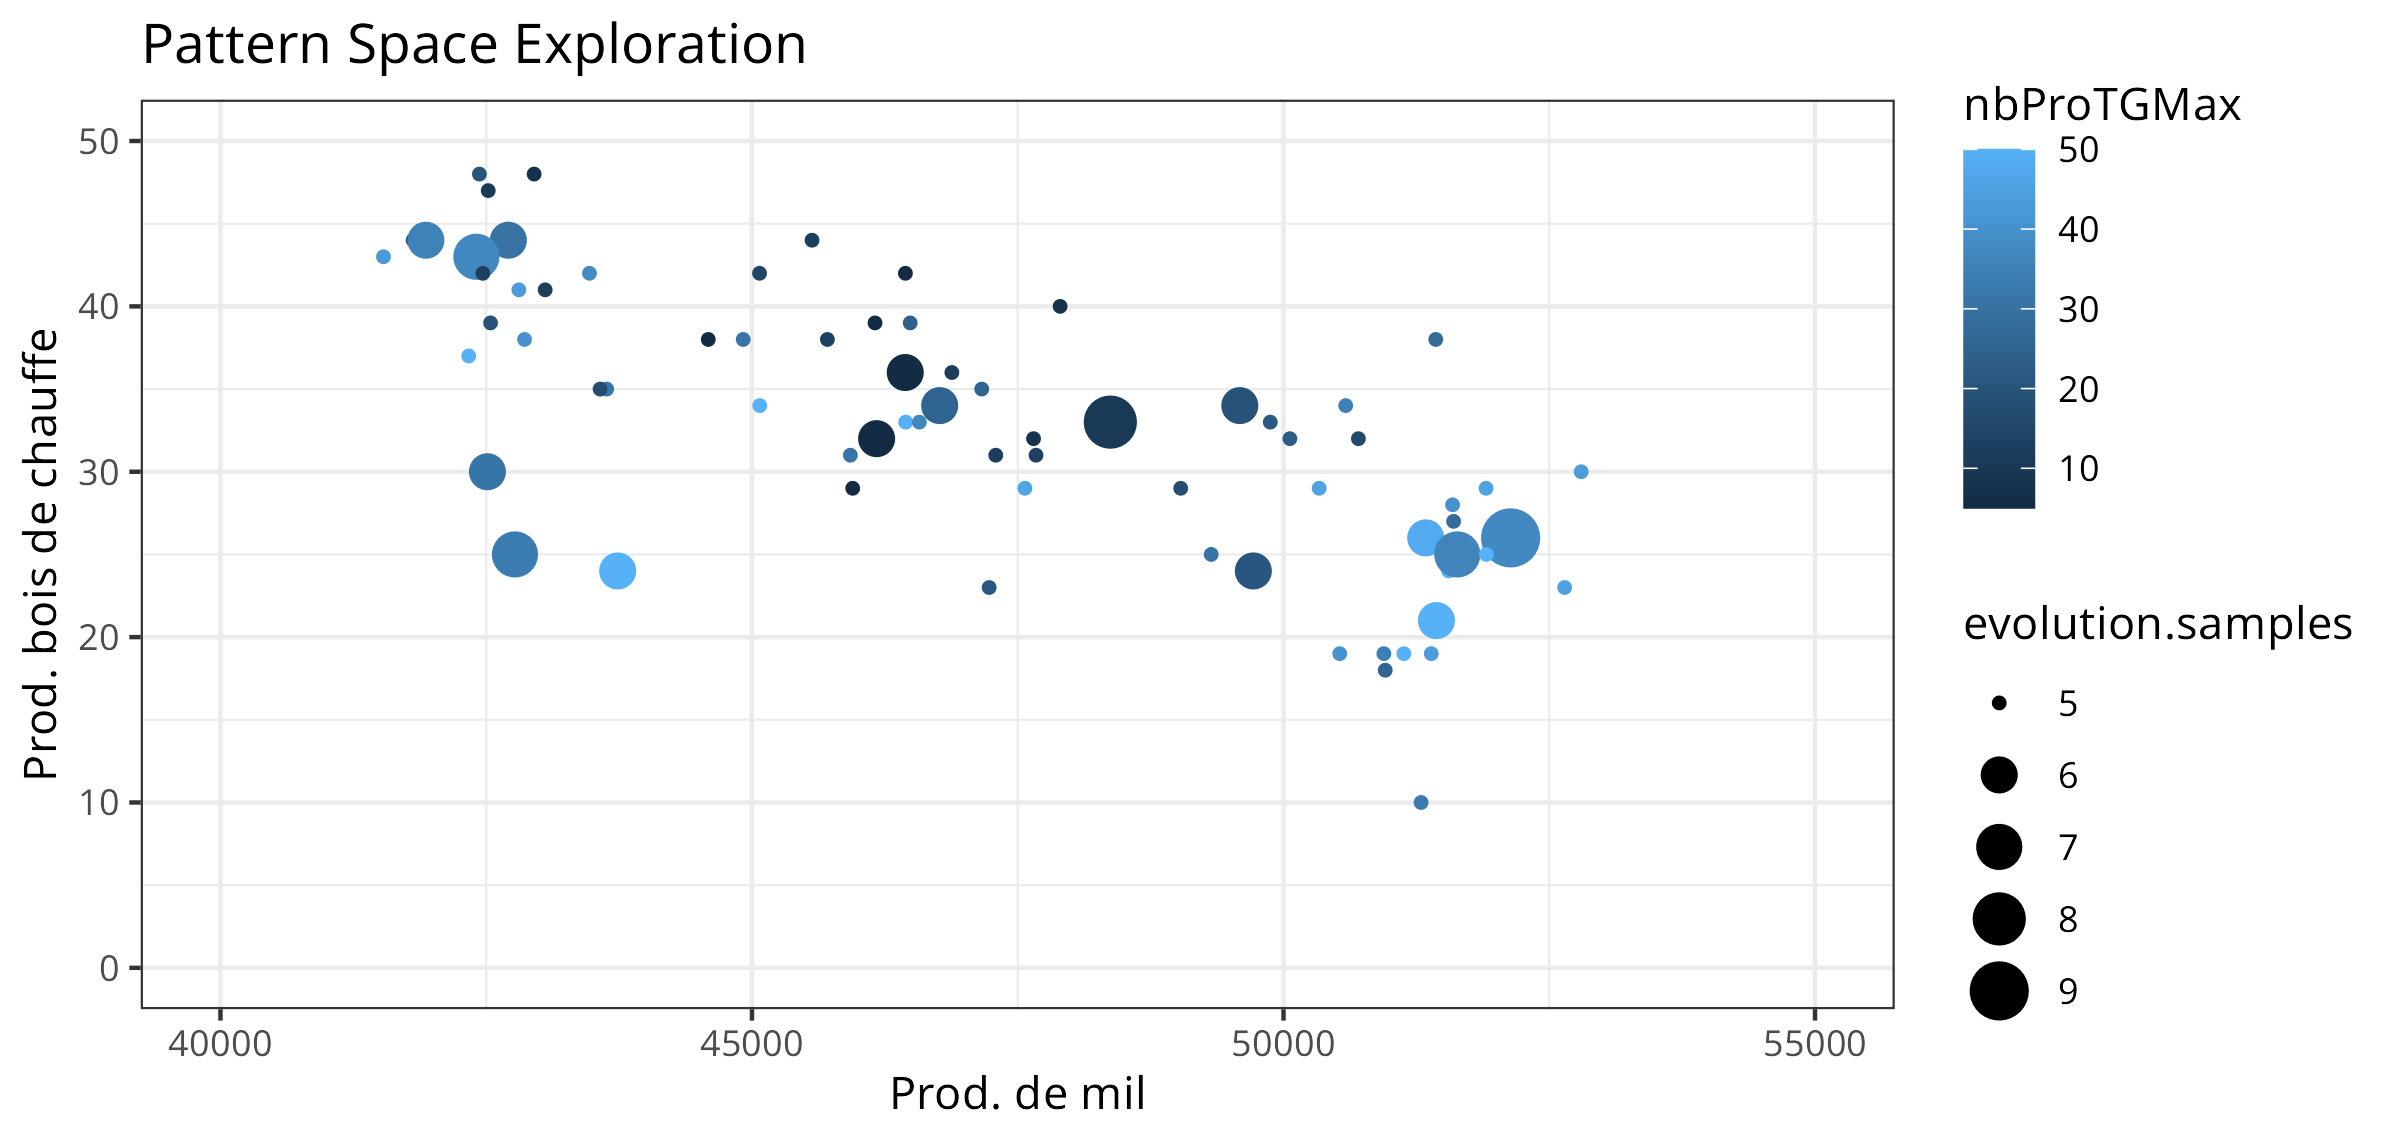
\includegraphics[width=\textwidth]{./img/om_pse.png}
            \caption{Résultat de 33600 évolutions de l'algorithme PSE. Chaque point est un résultat dans l'espace des sorties. La couleur met en évidence le nombre de jeunes pousses protégé par les agriculteurs, et la taille des points donne une idée de la "facilité" pour le modèle à atteindre cet espace. Plus un point est gros, plus le modèle arrive à l'atteindre.}
            \label{fig:PSE}
        \end{figure}

Viabilité du système 

% The results should describe the experiments performed and the findings observed. The results section should be divided into subsections to delineate different experimental themes. 
% \begin{itemize}
%     \item All data should be presented in the Results. No data should be presented for the first time in the Discussion. Data (such as from Western blots) should be appropriately quantified.
%     \item Subheadings must be either all complete sentences or all phrases. They should be brief, ideally less than 10 words. Subheadings should not end in a period. Your paper may have as many subheadings as are necessary.
%     \item Figures and tables must be called out in numerical order. For example, the first mention of any panel of Fig. 3 cannot precede the first mention of all panels of Fig. 2. The supplementary figures (for example, fig. S1) and tables (table S1) must also be called out in numerical order. 
% \end{itemize}

\section{Discussion}
Include a Discussion that summarizes (but does not merely repeat) your conclusions and elaborates on their implications. There should be a paragraph outlining the limitations of your results and interpretation, as well as a discussion of the steps that need to be taken for the findings to be applied. Please avoid claims of priority. 

\section*{Acknowledgments}

\subsection*{General} 
We warmly thank the residents of Diohine for their hospitality, with special thanks to: Aissatou Faye, Robert Diatte, Pierre Faye, Paul Sene, Ameth Paul Thiaw, Assane Diouf, Guedj Diouf, Nicolas Diouf, Ablaye Faye, Idrissa Faye, Maire-Hélène Ndjira Diouf, Seynabou Gakou, Joseph Sene, Ndeye Thiamal.

\subsection*{Author Contributions} 
Describe contributions of each author to the paper, using the first initial and full last name. 

``L. Broutin conceived the model and realize intervews.''

``E. Delay and L. Broutin animate multi-actor focus groups.''

``E. Delay conducte the HPC exploration.''

``E. Delay and L. Broutin realize the first draft of this manuscript.''

``All authors contributed equally to 2nd version of the manuscript.''

\subsection*{Funding}

This work is part of the research and development project DSCATT (Dynamics of Soil Carbon Sequestration in Tropical and Temperate Agricultural Systems, https://dscatt.net/FR/index.html) co-funded by Agropolis Fondation [reference ID 1802-001] through the "Investissements d'avenir" program Labex Agro [ANR-10-LABX-0001-01] within the framework of I-SITE MUSE [ANR-16-IDEX-0006] and supported by the TOTAL Energies Foundation.

\subsection*{Conflicts of Interest}
The author(s) declare(s) that there is no conflict of interest regarding the publication of this article.

\subsection*{Data Availability}
A data availability statement is compulsory for all research articles. This statement describes whether and how others can access the data supporting the findings of the paper, including 1) what the nature of the data is, 2) where the data can be accessed, and 3) any restrictions on data access and why.

If data are in an archive, include the accession number or a placeholder for it. Also include any materials that must be obtained through a Material Transfer Agreements (MTA). 

\section*{Supplementary Materials}
Describe any supplementary materials submitted with the manuscript (e.g., audio files, video clips or datasets). 

Please group supplementary materials in the following order: materials and methods, figures, tables, and other files (such as movies, data, interactive images, or database files). 

\medskip Example:
Fig. S1. Title of the first supplementary figure.

Fig. S2. Title of the second supplementary figure.

Table S1. Title of the first supplementary table.

Data file S1. Title of the first supplementary data file.

Movie S1. Title of the first supplementary movie.

\medskip
Be sure to submit all supplementary materials with the manuscript and remember to reference the supplementary materials at appropriate points within the manuscript. We recommend citing specific items, rather than referring to the supplementary materials in general, for example: ``See Figures S1-S10 in the Supplementary Material for comprehensive image analysis.''

A link to access the supplementary materials will be provided in the published article.

Supplementary Materials may include additional author notes—for example, a list of group authors.

\section*{Guidelines for References}

There is only one reference list for all sources cited in the main text, figure and table legends, and Supplementary Materials. Do not include a second reference list in the Supplementary Materials section. Include references cited only in the Supplementary Materials at the end of the reference section of the main text; reference numbering should continue as if the Supplementary Materials are a continuation of the main text. References cited only in the Supplementary Materials section are not counted toward length guidelines.

Authors are responsible for ensuring that the information in each reference is complete and accurate.

DOIs, if available, should be included for each reference.

Please do not include any extraneous language such as explanatory notes as part of a reference to a given source. The Journal of Remote Sensing prefers that manuscripts do not include end notes; if information is important enough to include, please put into main text.  If you need to include notes, please explain why they are needed in your cover letter to the editor.

\printbibliography

\end{document}
